\chapter{Complexe kinetiek: ketens, enzymen en oscillaties}\label{ch:b3:complex-kinetics}

Een beker met een geroerde oplossing wordt kleurloos, dan amberkleurig,
dan blauw, dan weer kleurloos, en blijft dat vele minuten lang herhalen;
uitgegoten in een schaal tekent hetzelfde mengsel spiralen die draaien en
zich verplaatsen. Toen Boris Belousov zo'n reactie in 1951 beschreef, werd
zijn manuscript geweigerd: een chemisch systeem, meende de referent, kan
niet heen en weer gaan, want het moet bergaf gaan naar het evenwicht. Het
gaat wel bergaf; het gaat alleen niet rechtdoor. Dit hoofdstuk behandelt
mechanismen met veel stappen waarvan de intermediairen geregenereerd
worden: \omterm{def:b3:complex-kinetics:chain}{kettingreacties} en explosies, moleculen die botsingen nodig hebben
om in hun eentje uiteen te vallen, \omterm{def:b3:complex-kinetics:enzyme}{enzymen}, en de \omterm{def:b3:complex-kinetics:oscillating}{oscillerende reacties},
met de methoden die reacties volgen die te snel zijn om met de hand te
mengen.

\begin{recall}
Het deel van jaar~1 definieerde een reactiemechanisme als een opeenvolging
van elementaire stappen, de snelheidsbepalende stap, de
voorevenwichtsbenadering en de stationaire-toestandsbenadering, en
katalysatoren. Het deel van jaar~2 benoemde de stappen van een
radicaalketen (initiatie, propagatie, terminatie), radicaalinitiatoren en
de kinetische ketenlengte van een polymerisatie, en paste
kleinstekwadratenrechten aan.
\Cref{ch:b3:rate-theories} gaf de \omterm{def:b3:rate-theories:tst}{overgangstoestandstheorie} en de
diffusielimiet van ongeveer \qty{e10}{L.mol^{-1}.s^{-1}}.
\end{recall}

\section{Kettingreacties}

\begin{definition}[Kettingreactie, kettingdrager]\label{def:b3:complex-kinetics:chain}
Een \emph{kettingreactie}\index{kettingreactie} is een reactie waarin
reactieve intermediairen, de \emph{kettingdragers}\index{kettingdrager},
geregenereerd worden door een cyclus van propagatiestappen, zodat één
initiatiegebeurtenis veel moleculen beginstof omzet.
\end{definition}

Bodenstein mat in 1906 de snelheid van $\ce{H2 + Br2 -> 2 HBr}$ en vond een
wet die geen enkele afzonderlijke stap kon voortbrengen: de snelheid
groeit als $[\ce{Br2}]^{1/2}$ en daalt naarmate HBr zich ophoopt. Het
mechanisme werd in 1919 opgeschreven:
\begin{center}
\begin{tabular}{lll}
initiatie & $\ce{Br2 -> 2 Br}$ & $k_1$ \\
propagatie & $\ce{Br + H2 -> HBr + H}$ & $k_2$ \\
propagatie & $\ce{H + Br2 -> HBr + Br}$ & $k_3$ \\
inhibitie & $\ce{H + HBr -> H2 + Br}$ & $k_4$ \\
terminatie & $\ce{2 Br -> Br2}$ & $k_{-1}$
\end{tabular}
\end{center}
(botsingen met een derde lichaam M, dat energie aanvoert naar en afvoert
uit de initiatie- en terminatiestappen, blijven impliciet).

\begin{theorem}[De snelheidswet van waterstof en broom]\label{thm:b3:complex-kinetics:hbr}
Met de stationaire-toestandsbenadering voor Br en H is de snelheid $v = \frac12\,\dd[\ce{HBr}]/\dd t$
van het mechanisme
\[
  v = \frac{k[\ce{H2}][\ce{Br2}]^{1/2}}{1 + k'[\ce{HBr}]/[\ce{Br2}]},
  \qquad k = k_2\Bigl(\frac{k_1}{k_{-1}}\Bigr)^{1/2},\ k' = \frac{k_4}{k_3}.
\]
\end{theorem}

\begin{proof}
Stationaire toestand voor H: $k_2[\ce{Br}][\ce{H2}] = k_3[\ce{H}][\ce{Br2}] + k_4[\ce{H}][\ce{HBr}]$. Stationaire toestand voor Br:
$2k_1[\ce{Br2}] - k_2[\ce{Br}][\ce{H2}] + k_3[\ce{H}][\ce{Br2}] + k_4[\ce{H}][\ce{HBr}] - 2k_{-1}[\ce{Br}]^2 = 0$. Als men de twee
vergelijkingen optelt, vallen de propagatietermen weg: $k_1[\ce{Br2}] = k_{-1}[\ce{Br}]^2$, dus $[\ce{Br}] =
(k_1/k_{-1})^{1/2}[\ce{Br2}]^{1/2}$. Dan is $[\ce{H}] = k_2[\ce{Br}][\ce{H2}]/(k_3[\ce{Br2}] + k_4[\ce{HBr}])$ en
\[
  \frac{\dd[\ce{HBr}]}{\dd t} = k_2[\ce{Br}][\ce{H2}] + k_3[\ce{H}][\ce{Br2}] - k_4[\ce{H}][\ce{HBr}] = 2k_3[\ce{H}][\ce{Br2}]
  = \frac{2k_2[\ce{Br}][\ce{H2}]}{1 + (k_4/k_3)[\ce{HBr}]/[\ce{Br2}]},
\]
met de eerste vergelijking; invullen van $[\ce{Br}]$ geeft het resultaat.
\end{proof}

\begin{omfigure}
\begin{tikzpicture}[font=\small, >=Stealth]
  \node[draw, circle, minimum size=9mm, omDef, thick] (br) at (0,0) {Br};
  \node[draw, circle, minimum size=9mm, omThm, thick] (h) at (4,0) {H};
  \draw[->, thick] (br) to[bend left=35] node[midway, above, align=center] {$+\,\ce{H2}$\\ $\to$ HBr} (h);
  \draw[->, thick] (h) to[bend left=35] node[midway, below, align=center] {$+\,\ce{Br2}$\\ $\to$ HBr} (br);
  \draw[->, thick, black!60] (-2.4,0) -- (br) node[pos=0, left, align=right] {initiatie\\ $\ce{Br2 -> 2 Br}$};
  \draw[->, thick, black!60] (br) -- (0,-2.0) node[below, align=center] {terminatie\\ $\ce{2 Br -> Br2}$};
  \draw[->, thick, black!60, dashed] (h) -- (6.2,-1.2) node[below, align=center] {inhibitie\\ $\ce{H + HBr -> H2 + Br}$};
\end{tikzpicture}

{\small De propagatiecyclus van de keten van waterstof en broom: elke
omloop verbruikt één \ce{H2} en één \ce{Br2}, maakt twee HBr en geeft het
broomatoom terug waarmee hij begon. De initiatie voedt de cyclus met
dragers, de terminatie verwijdert ze; de inhibitiestap zet een H-atoom
terug om in Br, ten koste van een HBr dat al gevormd was.}
\end{omfigure}

\begin{omfigure}
\begin{tikzpicture}
\begin{axis}[name=ca, width=0.47\linewidth, height=5.2cm, xmin=0, xmax=800, ymin=0, ymax=1,
  axis lines=left, xlabel={$t$ (gereduceerd)}, ylabel={$[\ce{HBr}]/2[\ce{H2}]_0$},
  tick label style={font=\small}, label style={font=\small}]
\addplot[omDef, thick] table[x=t, y expr=\thisrow{HBr}/2] {figdata/out/bachelor-3-chain-kinetics.dat};
\end{axis}
\begin{axis}[at={(ca.east)}, anchor=west, xshift=1.4cm, width=0.47\linewidth, height=5.2cm,
  xmin=0, xmax=60, ymin=0, ymax=2.2, axis lines=left, xlabel={$t$ (gereduceerd)},
  ylabel={snelheid $\times 10^3$}, tick label style={font=\small}, label style={font=\small},
  legend style={font=\scriptsize, draw=none, at={(0.97,0.03)}, anchor=south east},
  legend cell align=left]
\addplot[omDef, thick] table[x=t, y expr=1000*\thisrow{v}] {figdata/out/bachelor-3-chain-kinetics.dat};
\addplot[omThm, thick, dashed] table[x=t, y expr=1000*\thisrow{vss}] {figdata/out/bachelor-3-chain-kinetics.dat};
\legend{volledig mechanisme, wet van de stationaire toestand}
\end{axis}
\end{tikzpicture}

{\small Het mechanisme van waterstof en broom, stap voor stap
geïntegreerd (modelwaarden van de snelheidsconstanten, gereduceerde
eenheden, $k' = 0.1$): omzetting als functie van de tijd (links), en de
snelheid $\frac12\dd[\ce{HBr}]/\dd t$ van het volledige mechanisme vergeleken met de wet van
de stationaire toestand (rechts). Na een inductieperiode, waarin de
broomatomen zich opbouwen, vallen de twee samen tot op minder dan 1\,\%.}
\end{omfigure}

\begin{method}[De snelheidswet van een kettingmechanisme]\label{met:b3:complex-kinetics:steady-state-chain}
\begin{enumerate}
  \item Schrijf voor elke \omterm{def:b3:complex-kinetics:chain}{kettingdrager} een stationaire-toestandsvergelijking.
  \item Tel ze op: de propagatiestappen, die alleen de ene drager tegen de
        andere ruilen, vallen weg, en de initiatie blijft gelijk aan de
        terminatie; dat geeft de concentratie van de drager.
  \item Gebruik de vergelijking van één drager om de andere dragers uit te
        drukken.
  \item Schrijf de vormingssnelheid van een product uit de propagatiestappen.
\end{enumerate}
\end{method}

Het aantal propagatiecycli per initiatiegebeurtenis, hier $v/k_1[\ce{Br2}]$, is de
kinetische ketenlengte uit het deel van jaar~2; voor de reactie van
waterstof met broom is ze, afhankelijk van de omstandigheden, van de orde
van $10^3$ tot $10^6$. De inhibitie door het product verklaart waarom de
snelheid sneller daalt dan de beginstoffen verbruikt worden.

\section{Vertakte ketens en explosies}

\begin{definition}[Kettingvertakking, explosiegrenzen]\label{def:b3:complex-kinetics:branching}
\emph{Kettingvertakking}\index{kettingvertakking} is een propagatiestap
die meer \omterm{def:b3:complex-kinetics:chain}{kettingdragers} voortbrengt dan ze verbruikt, zoals $\ce{H + O2 -> OH + O}$, die van één
drager er twee maakt. De \emph{explosiegrenzen}\index{explosiegrenzen} van
een mengsel zijn de drukken waarbij, bij een gegeven temperatuur, zijn
trage reactie overgaat in een explosie.
\end{definition}

\begin{proposition}[Vertakkingscriterium]\label{prop:b3:complex-kinetics:branching}
Stel dat dragers ontstaan met de snelheid $v_i$, zich vermenigvuldigen door
vertakking met de snelheidsconstante $f$ en verdwijnen door terminatie met
de snelheidsconstante $g$:
$\dd n/\dd t = v_i + (f - g)n$. Als $f < g$, nadert $n$ tot de stationaire
waarde $v_i/(g - f)$; als
$f > g$, groeit $n$ exponentieel en explodeert de reactie.
\end{proposition}

\begin{proof}
De lineaire vergelijking heeft de oplossing $n(t) = \frac{v_i}{g - f}\bigl(1 - \eu^{-(g - f)t}\bigr)$, die
naar $v_i/(g - f)$ gaat wanneer $g > f$; wanneer $f > g$ is de exponent
positief en groeit $n$ als $\eu^{(f - g)t}$ zonder grens (tot de
beginstoffen op zijn).
\end{proof}

Voor mengsels van waterstof en zuurstof bij enkele honderden graden groeit
$f$ met de druk (het is evenredig met $[\ce{O2}]$), is de terminatie aan
de wanden van het vat snel bij lage druk (de radicalen diffunderen er
gemakkelijk naartoe), en groeit de terminatie door driedeeltjesbotsingen
($\ce{H + O2 + M -> HO2 + M}$) met het kwadraat van de druk. De vertakking
wint tussen een eerste grens, bepaald door de wanden, en een tweede grens,
bepaald door de driedeeltjesterminatie; bij nog hogere druk verschijnt een
derde grens waar de vrijgekomen warmte niet meer kan ontsnappen. Die
laatste is een thermische explosie, gedreven door de exponentiële groei
van de snelheid met de temperatuur in plaats van door vertakking; de
meeste industriële explosies zijn van dat soort.

\section{Monomoleculaire reacties}

Een molecuul zoals cyclopropaan isomeriseert in zijn eentje, met een
kinetiek van de eerste orde bij gewone drukken; toch daalt de
snelheidsconstante bij lage druk. De benodigde energie komt van botsingen.

\begin{definition}[Mechanisme van Lindemann, overgangsgebied]\label{def:b3:complex-kinetics:lindemann}
Het \emph{mechanisme van Lindemann}\index{mechanisme van Lindemann} van
een monomoleculaire reactie is de opeenvolging $\mathrm{A + M \rightleftharpoons A^* + M}$ ($k_1$, $k_{-1}$),
activering en deactivering door botsing met een willekeurig molecuul M,
gevolgd door $\mathrm{A^* \to P}$ ($k_2$). Het
\emph{overgangsgebied}\index{overgangsgebied} (``fall-off'') is het
drukbereik waarin de waargenomen snelheidsconstante van de eerste orde
daalt van haar waarde bij hoge druk naar een gedrag van de tweede orde.
\end{definition}

\begin{theorem}[Snelheidsconstante van Lindemann]\label{thm:b3:complex-kinetics:lindemann}
Met de stationaire-toestandsbenadering voor $\mathrm{A^*}$ is $v = k_{\mathrm{uni}}[\mathrm A]$ met
\[
  k_{\mathrm{uni}} = \frac{k_1k_2[\mathrm M]}{k_{-1}[\mathrm M] + k_2},
\]
die naar $k_\infty = k_1k_2/k_{-1}$ gaat bij hoge druk (eerste orde) en naar $k_1[\mathrm M]$ bij
lage druk (tweede orde); ze is $k_\infty/2$ bij $[\mathrm M]_{1/2} = k_2/k_{-1}$.
\end{theorem}

\begin{proof}
$\dd[\mathrm{A^*}]/\dd t = k_1[\mathrm A][\mathrm M] - k_{-1}[\mathrm{A^*}][\mathrm M] - k_2[\mathrm{A^*}] = 0$ geeft $[\mathrm{A^*}] =
k_1[\mathrm A][\mathrm M]/(k_{-1}[\mathrm M] + k_2)$ en $v = k_2[\mathrm{A^*}]$. Als $k_{-1}[\mathrm M] \gg k_2$, is de
deactivering sneller dan de reactie en is $\mathrm{A^*}$ in voorevenwicht: $k_{\mathrm{uni}} \to k_1k_2/k_{-1}$. Als $k_{-1}[\mathrm M]
\ll k_2$, reageert elk geactiveerd molecuul en is de activering
snelheidsbepalend:
$k_{\mathrm{uni}} \to k_1[\mathrm M]$.
\end{proof}

\begin{omfigure}
\begin{tikzpicture}
\begin{axis}[width=0.66\linewidth, height=5.4cm, xmode=log, ymode=log, xmin=1e-10, xmax=1e-2,
  ymin=1e-8, ymax=4e-3, axis lines=left, xlabel={$[\mathrm M]$ / \unit{mol.L^{-1}}},
  ylabel={$k_{\mathrm{uni}}$ / \unit{s^{-1}}}, tick label style={font=\small}, label style={font=\small}]
\addplot[black!40, dashed] table[x=M, y=low] {figdata/out/bachelor-3-lindemann.dat};
\addplot[black!40, dashed] table[x=M, y=high] {figdata/out/bachelor-3-lindemann.dat};
\addplot[omDef, very thick] table[x=M, y=k] {figdata/out/bachelor-3-lindemann.dat};
\node[font=\scriptsize, anchor=south, rotate=39] at (axis cs:4e-9,2.5e-5) {$k_1[\mathrm M]$};
\node[font=\scriptsize, anchor=south] at (axis cs:3e-4,1e-3) {$k_\infty$};
\draw[black!50, densely dotted] (axis cs:1e-6,1e-8) -- (axis cs:1e-6,5e-4);
\node[font=\scriptsize, anchor=north west] at (axis cs:1.2e-6,2e-7) {$[\mathrm M]_{1/2}$};
\end{axis}
\end{tikzpicture}

{\small De overgangskromme van Lindemann (modelconstanten): eerste orde met
de limietconstante $k_\infty$ bij hoge druk, tweede orde ($k_1[\mathrm M]$)
bij lage druk, en de helft van $k_\infty$ bij $[\mathrm M]_{1/2} = k_2/k_{-1}$.
Echte overgangskrommen zijn breder: de snelheidsconstante $k_2$ van een
aangeslagen molecuul groeit met zijn energie.}
\end{omfigure}

\section{Enzymkinetiek}

\begin{definition}[Enzym, actieve plaats, enzym-substraatcomplex]\label{def:b3:complex-kinetics:enzyme}
Een \emph{enzym}\index{enzym} is een biologische katalysator, bijna altijd
een eiwit, die een specifieke reactie van zijn substraat versnelt. De
\emph{actieve plaats}\index{actieve plaats} is de holte van het enzym waar
het substraat bindt en reageert; het gebonden deeltje is het
\emph{enzym-substraatcomplex}\index{enzym-substraatcomplex} ES.
\end{definition}

\begin{definition}[Michaelisconstante, maximale snelheid, katalytische constante en specificiteitsconstante]\label{def:b3:complex-kinetics:michaelis}
Voor het mechanisme $\mathrm{E + S \rightleftharpoons ES \to E + P}$ ($k_1$, $k_{-1}$, $k_2$) bij een totale enzymconcentratie
$[\mathrm E]_0$ is de
\emph{katalytische constante}\index{katalytische constante} $k_{\mathrm{cat}} = k_2$, de
\emph{maximale snelheid}\index{maximale snelheid} $V_{\max} = k_{\mathrm{cat}}[\mathrm E]_0$, de
\emph{michaelisconstante}
\index{michaelisconstante} $K_M = (k_{-1} + k_2)/k_1$, en de
\emph{specificiteitsconstante}
\index{specificiteitsconstante} $k_{\mathrm{cat}}/K_M$.
\end{definition}

\begin{theorem}[Vergelijking van Michaelis-Menten]\label{thm:b3:complex-kinetics:michaelis-menten}
Wanneer $[\mathrm S] \gg [\mathrm E]_0$ en ES zich in een stationaire
toestand bevindt, is de beginsnelheid van de vorming van het product
\[
  v = \frac{V_{\max}[\mathrm S]}{K_M + [\mathrm S]} .
\]
Deze uitspraak is de \emph{vergelijking van
Michaelis-Menten}\index{vergelijking van Michaelis-Menten}.
\end{theorem}

\begin{proof}
Stationaire toestand: $k_1[\mathrm E][\mathrm S] = (k_{-1} + k_2)[\mathrm{ES}]$, en $[\mathrm E] = [\mathrm E]_0 - [\mathrm{ES}]$ (het vrije
substraat is praktisch al het substraat, omdat $[\mathrm S] \gg [\mathrm E]_0$). Dus is $[\mathrm{ES}]
= [\mathrm E]_0[\mathrm S]/(K_M + [\mathrm S])$ en $v = k_2[\mathrm{ES}]$.
\end{proof}

\begin{remark}
Michaelis en Menten (1913) namen in plaats daarvan een snel voorevenwicht
aan van E, S en ES; dezelfde vergelijking volgt dan, met $K_M$ vervangen
door de dissociatieconstante $k_{-1}/k_1$, de limiet van $K_M$ wanneer $k_2 \ll k_{-1}$. De
\omterm{def:b3:complex-kinetics:michaelis}{katalytische constante} is wat biochemici het omzetgetal van het \omterm{def:b3:complex-kinetics:enzyme}{enzym}
noemen: het aantal substraatmoleculen dat één \omterm{def:b3:complex-kinetics:enzyme}{actieve plaats} per seconde
omzet wanneer ze verzadigd is.
\end{remark}

Bij $[\mathrm S] = K_M$ is de snelheid $V_{\max}/2$; bij $[\mathrm S] \ll K_M$ is ze $(k_{\mathrm{cat}}/K_M)[\mathrm E]_0[\mathrm S]$: de
\omterm{def:b3:complex-kinetics:michaelis}{specificiteitsconstante} is de snelheidsconstante van de tweede orde van
het vrije \omterm{def:b3:complex-kinetics:enzyme}{enzym} met zijn substraat, en ze kan de snelheid waarmee die
elkaar ontmoeten niet overschrijden, de diffusielimiet van
\cref{ch:b3:rate-theories}. Enkele \omterm{def:b3:complex-kinetics:enzyme}{enzymen} komen er dichtbij; het
``gemiddelde'' \omterm{def:b3:complex-kinetics:enzyme}{enzym}, in een overzicht van enkele duizenden, heeft een $k_{\mathrm{cat}}/K_M$ van ongeveer
$10^5$~\unit{L.mol^{-1}.s^{-1}}, zo'n vier grootteordes lager.

\begin{proposition}[Vorm van Lineweaver-Burk]\label{prop:b3:complex-kinetics:lineweaver}
De \omterm{thm:b3:complex-kinetics:michaelis-menten}{vergelijking van Michaelis-Menten} is gelijkwaardig met
\[
  \frac1v = \frac{1}{V_{\max}} + \frac{K_M}{V_{\max}}\,\frac{1}{[\mathrm S]},
\]
een rechte van $1/v$ tegen $1/[\mathrm S]$ met afsnijding $1/V_{\max}$,
helling $K_M/V_{\max}$, en
afsnijding $-1/K_M$ op de as $1/[\mathrm S]$.
\end{proposition}

\begin{proof}
Neem het omgekeerde: $1/v = (K_M + [\mathrm S])/(V_{\max}[\mathrm S])$. Bij $1/v = 0$ is $1/[\mathrm S] = -1/K_M$.
\end{proof}

\begin{method}[$K_M$ en $V_{\max}$ met niet-lineaire kleinste kwadraten]\label{met:b3:complex-kinetics:mm-fit}
\begin{enumerate}
  \item Meet beginsnelheden bij substraatconcentraties gespreid van
        ongeveer
        $K_M/5$ tot $10K_M$.
  \item Pas $v = V_{\max}[\mathrm S]/(K_M + [\mathrm S])$ rechtstreeks aan, door $\sum(v_i - v(\mathrm S_i))^2$ te minimaliseren (iteratief,
        vertrekkend van de waarden van een rechte van Lineweaver-Burk); de
        standaardfouten volgen uit de residuen en de gevoeligheid van $v$
        voor elke parameter.
  \item Gebruik de grafiek van Lineweaver-Burk alleen om het patroon te
        zien: het omkeren van kleine snelheden vergroot hun fouten, zodat
        de kleinstekwadratenrechte door $1/v$ gedomineerd wordt door de
        minst nauwkeurige punten, en haar parameters vertekend zijn.
\end{enumerate}
\end{method}

\begin{definition}[Inhibitie]\label{def:b3:complex-kinetics:inhibition}
Een inhibitor I bindt omkeerbaar aan het \omterm{def:b3:complex-kinetics:enzyme}{enzym}. Bij \emph{competitieve
inhibitie}\index{competitieve inhibitie} bindt hij alleen aan het vrije
\omterm{def:b3:complex-kinetics:enzyme}{enzym}, in de \omterm{def:b3:complex-kinetics:enzyme}{actieve plaats}, met de
\emph{inhibitieconstante}\index{inhibitieconstante} $K_i$
(dissociatieconstante van EI); bij
\emph{oncompetitieve inhibitie}\index{oncompetitieve inhibitie}
bindt hij alleen aan ES, met de constante $K_i'$; bij \emph{gemengde
inhibitie}\index{gemengde inhibitie} bindt hij aan beide.
\end{definition}

\begin{proposition}[Snelheidswetten met inhibitie]\label{prop:b3:complex-kinetics:inhibition-laws}
Met $\alpha = 1 + [\mathrm I]/K_i$ en $\alpha' = 1 + [\mathrm I]/K_i'$ behoudt de snelheid de
vorm van Michaelis-Menten $v = V^{\mathrm{app}}[\mathrm S]/(K_M^{\mathrm{app}} + [\mathrm S])$, met: competitief
$K_M^{\mathrm{app}} = \alpha K_M$, $V^{\mathrm{app}} = V_{\max}$; oncompetitief $K_M^{\mathrm{app}} = K_M/\alpha'$, $V^{\mathrm{app}} =
V_{\max}/\alpha'$; gemengd $K_M^{\mathrm{app}} = \alpha K_M/\alpha'$, $V^{\mathrm{app}} = V_{\max}/\alpha'$.
\end{proposition}

\begin{proof}
Gemengd geval (de andere zijn er de limieten $K_i' \to \infty$ en $K_i \to \infty$ van): het \omterm{def:b3:complex-kinetics:enzyme}{enzym}
is verdeeld over E, EI, ES en ESI met $[\mathrm{EI}] = [\mathrm E][\mathrm I]/K_i$, $[\mathrm{ESI}] = [\mathrm{ES}][\mathrm I]/K_i'$
en de stationaire toestand $[\mathrm E][\mathrm S] = K_M[\mathrm{ES}]$. Dus is $[\mathrm E]_0 = [\mathrm E]\alpha + [\mathrm{ES}]\alpha' =
[\mathrm{ES}](\alpha K_M/[\mathrm S] + \alpha')$ en $v = k_2[\mathrm{ES}] = V_{\max}[\mathrm S]/(\alpha K_M + \alpha'[\mathrm S])$; teller
en noemer delen door $\alpha'$ geeft de vermelde vorm.
\end{proof}

\begin{method}[Het type inhibitie herkennen]\label{met:b3:complex-kinetics:inhibition-type}
\begin{enumerate}
  \item Meet $v([\mathrm S])$ bij verschillende inhibitorconcentraties en
        teken de rechten van Lineweaver-Burk.
  \item Rechten die elkaar snijden op de as $1/v$ (dezelfde $V_{\max}$):
        competitief; een grote overmaat substraat overwint de inhibitor.
  \item Evenwijdige rechten (helling $K_M/V_{\max}$ onveranderd): oncompetitief.
  \item Rechten die elkaar links van de as $1/v$ snijden: gemengd.
  \item Bepaal $K_i$ door de schijnbare constanten uit te zetten tegen
        $[\mathrm I]$: voor een competitieve inhibitor is $K_M^{\mathrm{app}} = K_M + (K_M/K_i)[\mathrm I]$ een rechte.
\end{enumerate}
\end{method}

\begin{omfigure}
\begin{tikzpicture}
\begin{axis}[name=mv, width=0.47\linewidth, height=5.4cm, xmin=0, xmax=8, ymin=0, ymax=0.55,
  axis lines=left, xlabel={$[\mathrm S]$ / mM}, ylabel={$v$ / \unit{\micro M.s^{-1}}},
  tick label style={font=\small}, label style={font=\small},
  legend style={font=\scriptsize, draw=none, fill=white, fill opacity=0.85, text opacity=1,
  at={(0.97,0.03)}, anchor=south east}, legend cell align=left]
\addplot[black, thick] table[x=S, y=none] {figdata/out/bachelor-3-michaelis-menten-model.dat};
\addplot[omDef, thick] table[x=S, y=comp] {figdata/out/bachelor-3-michaelis-menten-model.dat};
\addplot[omThm, thick] table[x=S, y=uncomp] {figdata/out/bachelor-3-michaelis-menten-model.dat};
\draw[black!40, densely dotted] (axis cs:0,0.25) -- (axis cs:0.8,0.25) -- (axis cs:0.8,0);
\node[font=\scriptsize, anchor=north west] at (axis cs:0.85,0.12) {$K_M$};
\legend{zonder inhibitor, competitief, oncompetitief}
\end{axis}
\begin{axis}[at={(mv.east)}, anchor=west, xshift=1.5cm, width=0.47\linewidth, height=5.4cm,
  xmin=-2.5, xmax=3.5, ymin=0, ymax=12, axis x line=middle, axis y line=middle,
  tick label style={font=\small}, xtick={-2,-1,1,2,3}]
\node[font=\small, anchor=south east] at (axis cs:3.5,0.3) {$1/[\mathrm S]$};
\node[font=\small, anchor=north west] at (axis cs:0.12,12) {$1/v$};
\addplot[black, thick, domain=-1.25:3.5] {1.6*x + 2};
\addplot[omDef, thick, domain=-0.4167:3.5] {4.8*x + 2};
\addplot[omThm, thick, domain=-2.5:3.5] {1.6*x + 4};
\end{axis}
\end{tikzpicture}

{\small Kinetiek van Michaelis-Menten met $K_M = \qty{0.80}{mM}$ en $V_{\max} = \qty{0.50}{\micro M.s^{-1}}$
(model): zonder inhibitor (zwart), een competitieve inhibitor bij $[\mathrm I] = 2K_i$ (blauw,
$K_M$ verdrievoudigd, dezelfde $V_{\max}$) en een oncompetitieve bij $[\mathrm I] = K_i'$ (rood, $K_M$ en
$V_{\max}$ gehalveerd). Rechts: de rechten van Lineweaver-Burk; de
competitieve rechte snijdt de niet-geïnhibeerde op de as $1/v$, de
oncompetitieve loopt er evenwijdig mee
($1/[\mathrm S]$ in \unit{mM^{-1}}, $1/v$ in \unit{s.\micro M^{-1}}).}
\end{omfigure}

\section{Autokatalyse, oscillaties en snelle reacties}

\begin{definition}[Autokatalytische reactie]\label{def:b3:complex-kinetics:autocatalysis}
Een \emph{autokatalytische reactie}\index{autokatalytische reactie} is een
reactie waarin een product zijn eigen vorming katalyseert, zoals in $\mathrm{A + X \to 2\,X}$.
\end{definition}

\begin{proposition}[Logistische wet]\label{prop:b3:complex-kinetics:logistic}
Voor $\mathrm{A + X \to 2\,X}$ met snelheidsconstante $k$ en
beginconcentraties $a_0$ en $x_0$, met $N = a_0 + x_0$, is
\[
  x(t) = \frac{N}{1 + (N/x_0 - 1)\eu^{-kNt}},
\]
een S-vormige kromme die de helft van haar eindwaarde bereikt bij $t_{1/2} = \ln(N/x_0 - 1)/kN$.
\end{proposition}

\begin{proof}
$\dd x/\dd t = kx(N - x)$, omdat $a = N - x$. Scheiden van de
veranderlijken geeft $\frac{\dd x}{x(N - x)} = \frac1N\bigl(\frac1x + \frac{1}{N - x}\bigr)\dd x
= k\,\dd t$, dus $\ln\frac{x}{N - x} = kNt + \ln\frac{x_0}{N - x_0}$, wat
herschikt de vermelde vorm geeft;
$x = N/2$ wanneer $(N/x_0 - 1)\eu^{-kNt} = 1$.
\end{proof}

\begin{definition}[Oscillerende reactie, limietcyclus]\label{def:b3:complex-kinetics:oscillating}
Een \emph{oscillerende reactie}\index{oscillerende reactie} is een reactie
waarin de concentraties van intermediairen periodiek stijgen en dalen
terwijl de totale reactie naar het evenwicht voortschrijdt. Een
\emph{limietcyclus}\index{limietcyclus} is een gesloten baan in de ruimte
van de concentraties waar naburige banen naar convergeren, zodat de
oscillatie een amplitude heeft die niet van het beginpunt afhangt.
\end{definition}

\begin{theorem}[Model van Lotka-Volterra]\label{thm:b3:complex-kinetics:lotka-volterra}
Voor het autokatalytische schema $\mathrm{A + X \to 2\,X}$, $\mathrm{X + Y \to 2\,Y}$, $\mathrm{Y \to B}$ met A
constant gehouden, gehoorzamen de concentraties aan $\dot x = x(a - by)$, $\dot y = y(dx - c)$ met
positieve constanten, en de grootheid
\[
  V = dx - c\ln x + by - a\ln y
\]
is constant langs elke baan: de banen zijn gesloten krommen rond de
stationaire toestand $(c/d, a/b)$, en de concentraties oscilleren met een
amplitude die vastgelegd wordt door het beginpunt.
\end{theorem}

\begin{proof}
$\dot V = (d - c/x)\dot x + (b - a/y)\dot y = (dx - c)(a - by) + (by - a)(dx - c) = 0$. $V$ is een
som van twee convexe functies met één enkel minimum in $(c/d, a/b)$, zodat
haar niveaukrommen gesloten krommen rond dat punt zijn; een baan blijft op
een ervan en loopt er, omdat de snelheid elders nooit nul wordt,
periodiek rond.
\end{proof}

De oscillaties van Lotka-Volterra zijn kwetsbaar: elk beginpunt geeft zijn
eigen baan, en elke verstoring brengt het systeem naar een andere. Echte
chemische oscillatoren hebben een \omterm{def:b3:complex-kinetics:oscillating}{limietcyclus}, waarvoor een
niet-lineariteit nodig is die de stationaire toestand destabiliseert.

\begin{proposition}[Instabiliteit van de brusselator]\label{prop:b3:complex-kinetics:hopf}
Het model $\dot X = A - (B + 1)X + X^2Y$, $\dot Y = BX - X^2Y$ (gereduceerde concentraties,
$A$ en $B$ constant gehouden) heeft de enige stationaire toestand $(A, B/A)$, die
stabiel is als $B < 1 + A^2$ en instabiel als $B > 1 + A^2$; het systeem
komt dan op een \omterm{def:b3:complex-kinetics:oscillating}{limietcyclus} terecht.
\end{proposition}

\begin{proof}
Beide afgeleiden nul stellen: $BX = X^2Y$ geeft $XY = B$, en dan $A - X = 0$. De
jacobimatrix in $(A, B/A)$ is
\[
  \begin{pmatrix} -(B + 1) + 2XY & X^2 \\ B - 2XY & -X^2 \end{pmatrix}
  = \begin{pmatrix} B - 1 & A^2 \\ -B & -A^2 \end{pmatrix},
\]
met spoor $B - 1 - A^2$ en determinant $A^2 > 0$. Kleine afwijkingen
evolueren als
$\eu^{\lambda t}$ met $\lambda$ de \omterm{def:b3:quantum-model-systems:operator}{eigenwaarden}, waarvan het product de
determinant is (positief) en de som het spoor: beide hebben een negatief
reëel deel wanneer het spoor negatief is, een positief reëel deel wanneer
het positief is. Het bestaan van de \omterm{def:b3:complex-kinetics:oscillating}{limietcyclus} voor $B > 1 + A^2$ (de
banen blijven opgesloten in een begrensd gebied) wordt aangenomen.
\end{proof}

\begin{method}[De lineaire stabiliteit van een stationaire toestand]\label{met:b3:complex-kinetics:stability}
\begin{enumerate}
  \item Zoek de stationaire toestand door alle tijdsafgeleiden nul te stellen.
  \item Bereken daar de jacobimatrix van de partiële afgeleiden van de snelheden.
  \item Voor twee veranderlijken: stabiel als het spoor negatief is en de
        determinant positief; een instabiele toestand met complexe
        \omterm{def:b3:quantum-model-systems:operator}{eigenwaarden}
        ($\mathrm{tr}^2 < 4\det$) geeft groeiende oscillaties, een \omterm{def:b3:complex-kinetics:oscillating}{kandidaat-limietcyclus}.
\end{enumerate}
\end{method}

\begin{omfigure}
\begin{tikzpicture}
\begin{axis}[name=bs, width=0.62\linewidth, height=4.6cm, xmin=0, xmax=40, ymin=0, ymax=5.2,
  axis lines=left, xlabel={$t$ (gereduceerd)}, ylabel={concentratie},
  tick label style={font=\small}, label style={font=\small},
  legend style={font=\scriptsize, draw=none, at={(1.03,0.98)}, anchor=north west}]
\addplot[omDef, thick] table[x=t, y=X] {figdata/out/bachelor-3-oscillations-series.dat};
\addplot[omThm, thick] table[x=t, y=Y] {figdata/out/bachelor-3-oscillations-series.dat};
\legend{$X$, $Y$}
\end{axis}
\begin{axis}[name=ph, at={(bs.below south west)}, anchor=north west, yshift=-0.6cm,
  width=0.42\linewidth, height=5.0cm, xmin=0, xmax=4.8, ymin=0, ymax=5.6, axis lines=left,
  xlabel={$X$}, ylabel={$Y$}, tick label style={font=\small}, label style={font=\small},
  title={\small Brusselator}]
\addplot[omDef, thin] table[x=X, y=Y] {figdata/out/bachelor-3-oscillations-inner.dat};
\addplot[omThm, thin] table[x=X, y=Y] {figdata/out/bachelor-3-oscillations-outer.dat};
\addplot[only marks, mark=*, mark size=1.5pt] coordinates {(1,3)};
\end{axis}
\begin{axis}[at={(ph.east)}, anchor=west, xshift=1.3cm, width=0.42\linewidth, height=5.0cm,
  xmin=0, xmax=3.2, ymin=0, ymax=3.2, axis lines=left, xlabel={$x$}, ylabel={$y$},
  tick label style={font=\small}, label style={font=\small}, title={\small Lotka--Volterra}]
\addplot[black!70, thick] table[x=x, y=y] {figdata/out/bachelor-3-oscillations-lv1.dat};
\addplot[omDef, thick] table[x=x, y=y] {figdata/out/bachelor-3-oscillations-lv2.dat};
\addplot[omThm, thick] table[x=x, y=y] {figdata/out/bachelor-3-oscillations-lv3.dat};
\addplot[only marks, mark=*, mark size=1.5pt] coordinates {(1,1)};
\end{axis}
\end{tikzpicture}

{\small Boven: de brusselator ($A = 1$, $B = 3 > 1 + A^2$) komt terecht in
blijvende oscillaties met periode 7.2 (gereduceerde tijd). Linksonder: twee
banen, één die start dicht bij de instabiele stationaire toestand (stip)
en één ver daarbuiten, wikkelen zich op dezelfde \omterm{def:b3:complex-kinetics:oscillating}{limietcyclus}. Rechtsonder:
banen van Lotka-Volterra, elk vastgelegd door haar beginpunt, rond de
stationaire toestand (stip).}
\end{omfigure}

De reactie van Belousov-Zhabotinsky, de oxidatie van malonzuur door
bromaat, gekatalyseerd door cerium of door een ferroïne-indicator,
doorloopt zo'n cyclus: een autokatalytische productie van \ce{HBrO2}
schakelt in wanneer bromide onder een drempel zakt, oxideert de
katalysator (de kleuromslag), en wordt uitgeschakeld wanneer de
geoxideerde katalysator bromide regenereert. Zonder roeren, in een dunne
laag, plant de oscillatie zich voort als golven.

\begin{omfigure}
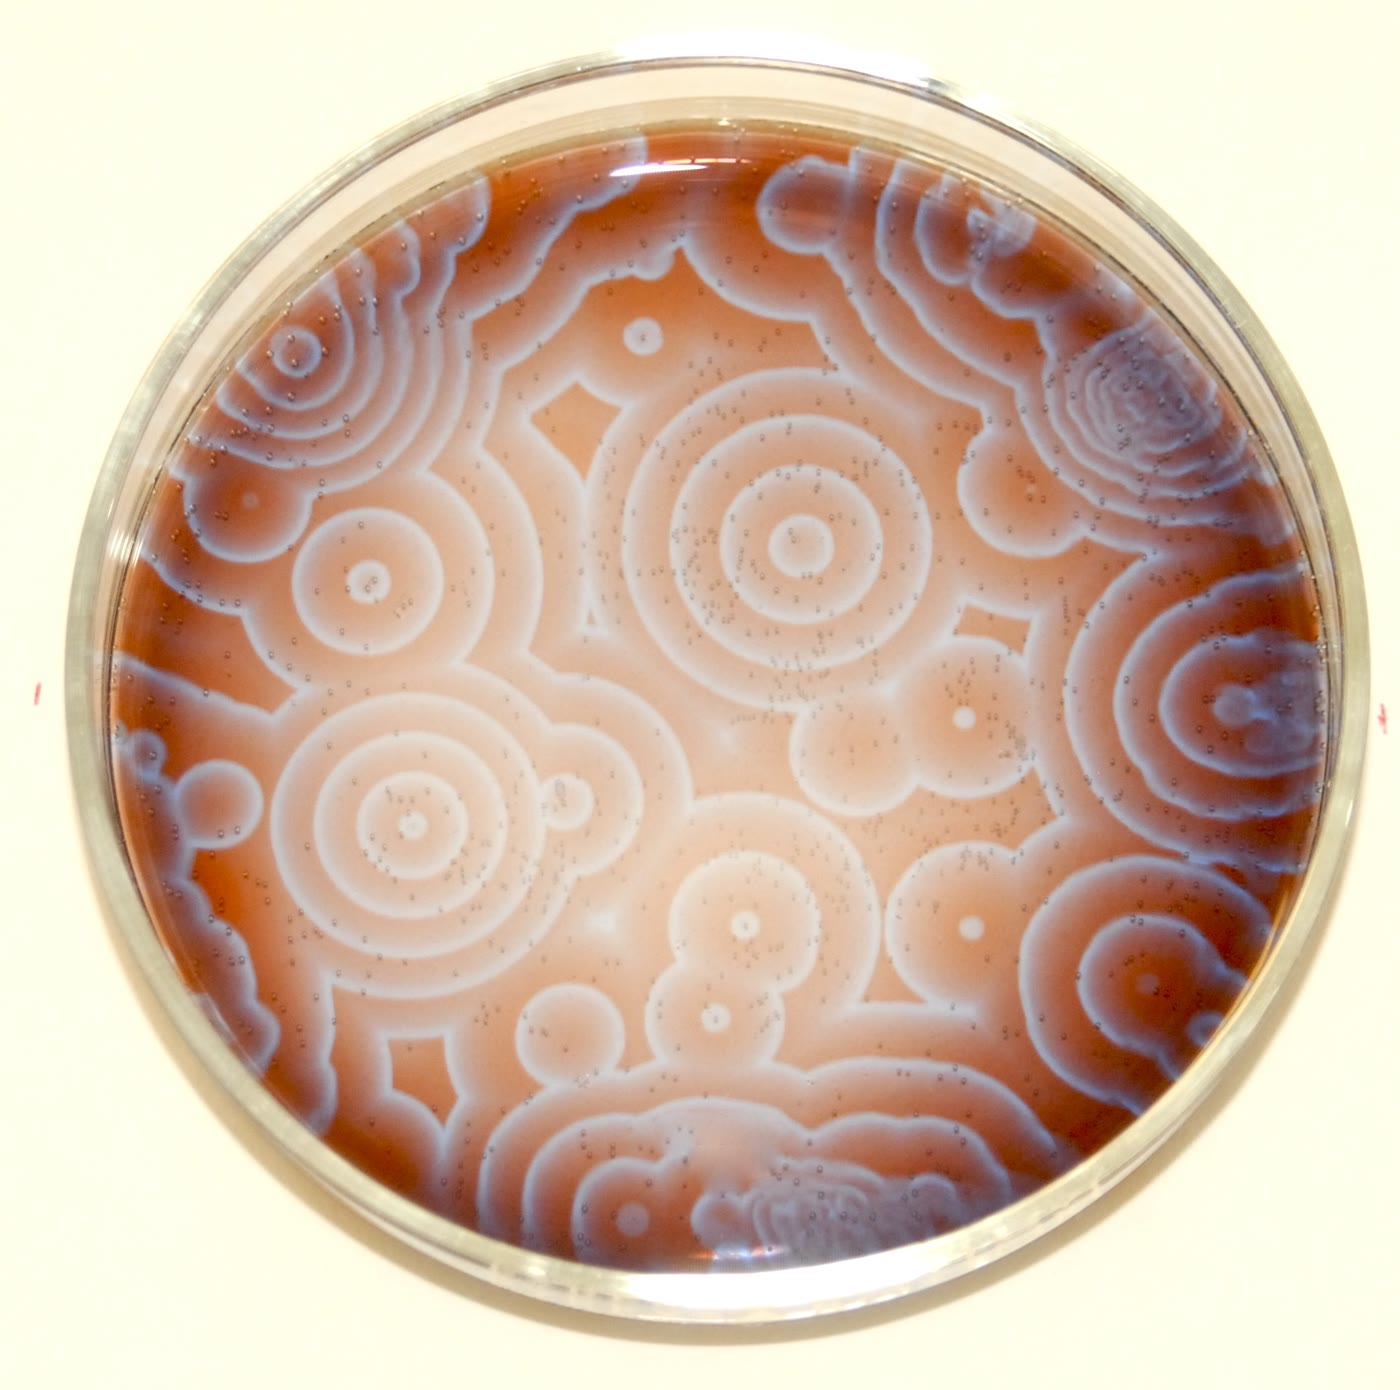
\includegraphics[width=0.48\linewidth]{images/book4/bz-reaction.jpg}

{\small Spiraalgolven van de reactie van Belousov-Zhabotinsky in een dunne
laag oplossing: elk blauw front is een oxidatiegolf van de katalysator,
die zich voortplant in het gereduceerde (rode) medium en niet kan
terugkeren in het gebied dat ze net verlaten heeft.}
\end{omfigure}

\begin{definition}[Relaxatiemethode, chemische relaxatietijd]\label{def:b3:complex-kinetics:relaxation}
Een \emph{relaxatiemethode}\index{relaxatiemethode} verstoort een systeem
in evenwicht plotseling (door een sprong van temperatuur, druk of
elektrisch veld) en volgt zijn terugkeer naar het nieuwe evenwicht. Bij
een kleine verstoring vervalt de afwijking exponentieel, met de
\emph{chemische relaxatietijd}\index{chemische relaxatietijd} $\tau$.
\end{definition}

\begin{proposition}[Relaxatietijd van een associatie]\label{prop:b3:complex-kinetics:relaxation-time}
Voor $\mathrm{A + B \rightleftharpoons C}$ ($k_1$, $k_{-1}$) is na een kleine verstoring
\[
  \frac1\tau = k_1([\mathrm A]_e + [\mathrm B]_e) + k_{-1} .
\]
\end{proposition}

\begin{proof}
Schrijf $[\mathrm C] = [\mathrm C]_e + x$, $[\mathrm A] = [\mathrm A]_e - x$, $[\mathrm B] = [\mathrm B]_e - x$. Dan is $\dot x =
k_1([\mathrm A]_e - x)([\mathrm B]_e - x) - k_{-1}([\mathrm C]_e + x)$; de termen zonder $x$ vallen
weg in het evenwicht, en na weglating van $x^2$: $\dot x = -[k_1([\mathrm A]_e + [\mathrm B]_e) + k_{-1}]x$.
\end{proof}

Het meten van $\tau$ bij verschillende concentraties geeft een rechte van $1/\tau$ tegen $[\mathrm A]_e +
[\mathrm B]_e$ met helling $k_1$ en afsnijding $k_{-1}$: beide constanten
uit experimenten op een systeem dat nooit meer dan enkele procenten van
het evenwicht afwijkt. Manfred Eigen mat op deze manier de snelste
reacties in oplossing, waaronder de neutralisatie van \ce{H3O+} door \ce{OH-}.

\begin{omfigure}
\begin{tikzpicture}
\begin{axis}[width=0.62\linewidth, height=5.0cm, xmin=0, xmax=780, ymin=0, ymax=1.05,
  axis lines=left, xlabel={$t$ / \unit{\micro s}}, ylabel={$([\mathrm C] - [\mathrm C]_e)/([\mathrm C]_0 - [\mathrm C]_e)$},
  tick label style={font=\small}, label style={font=\small},
  legend style={font=\scriptsize, draw=none, at={(0.97,0.97)}, anchor=north east},
  legend cell align=left]
\addplot[omDef, very thick] table[x=t_us, y=dC] {figdata/out/bachelor-3-chemical-relaxation.dat};
\addplot[omThm, thick, dashed] table[x=t_us, y=exp] {figdata/out/bachelor-3-chemical-relaxation.dat};
\legend{volledige snelheidsvergelijking, {$\eu^{-t/\tau}$, $\tau = \qty{156}{\micro s}$}}
\draw[black!40, densely dotted] (axis cs:156,0) -- (axis cs:156,0.368) -- (axis cs:0,0.368);
\end{axis}
\end{tikzpicture}

{\small Relaxatie van $\mathrm{A + B \rightleftharpoons C}$ na een
temperatuursprong die de evenwichtsconstante met 5\,\% verlaagde (model:
$k_1 = \qty{1.0e8}{L.mol^{-1}.s^{-1}}$, $k_{-1} = \qty{1.0e3}{s^{-1}}$,
\qty{1.0e-4}{mol/L} aan A en B in totaal): de volledige
snelheidsvergelijking en de exponentiële functie met
$1/\tau = k_1([\mathrm A]_e + [\mathrm B]_e) + k_{-1}$ vallen samen.}
\end{omfigure}

\begin{definition}[Stopped flow, flitsfotolyse]\label{def:b3:complex-kinetics:fast}
De \emph{stopped-flowmethode}\index{stopped-flowmethode} mengt twee
oplossingen van beginstoffen in ongeveer een milliseconde door ze via een
menger in een meetcel te drijven, stopt dan de stroming en registreert de
absorbantie of de \omterm{def:b3:electronic-spectroscopy:luminescence}{fluorescentie}.
\emph{Flitsfotolyse}\index{flitsfotolyse} maakt een reactief deeltje met
een korte, intense lichtpuls en volgt zijn reacties met een tweede,
vertraagde lichtbundel.
\end{definition}

\begin{omfigure}
\begin{tikzpicture}[font=\small, >=Stealth]
  % two drive syringes
  \foreach \y/\lab in {1.1/A, -0.1/B}{
    \draw[thick] (0,\y) rectangle (2.2,\y+0.6);
    \fill[omDef!25] (0.6,\y+0.05) rectangle (2.15,\y+0.55);
    \draw[thick] (0.6,\y) -- (0.6,\y+0.6);
    \draw[thick] (-0.6,\y+0.3) -- (0.6,\y+0.3);
    \node at (1.4,\y+0.3) {\lab};
    \draw[thick] (2.2,\y+0.3) -- (2.8,\y+0.3);}
  \draw[thick] (2.8,1.4) -- (3.2,0.8) (2.8,0.2) -- (3.2,0.8);
  \node[draw, thick, circle, minimum size=5mm, fill=white] (mx) at (3.4,0.8) {};
  \node[font=\scriptsize, anchor=north] at (3.4,0.5) {menger};
  \draw[thick] (mx.east) -- (4.4,0.8);
  \draw[thick, fill=omThm!15] (4.4,0.55) rectangle (5.4,1.05);
  \node[font=\scriptsize, anchor=north west, align=left] at (5.0,0.5) {meetcel};
  \draw[->, omThm, thick] (4.9,2.0) -- (4.9,1.1) node[pos=0, above, font=\scriptsize] {licht};
  \draw[->, omThm, thick] (4.9,0.5) -- (4.9,-0.4) node[below, font=\scriptsize] {detector};
  \draw[thick] (5.4,0.8) -- (6.2,0.8);
  \draw[thick] (6.2,0.5) rectangle (7.6,1.1);
  \draw[thick] (7.0,0.5) -- (7.0,1.1);
  \draw[thick] (7.0,0.8) -- (7.9,0.8);
  \draw[thick] (7.9,0.4) -- (7.9,1.2);
  \node[font=\scriptsize, anchor=south] at (6.9,1.15) {stopspuit};
  \draw[->, black!60] (-1.2,1.4) -- (-0.7,1.4) node[pos=0, left, font=\scriptsize] {aandrijving};
  \draw[->, black!60] (-1.2,0.2) -- (-0.7,0.2);
\end{tikzpicture}

{\small Een stopped-flowtoestel. De aandrijving duwt op twee spuiten; de
oplossingen ontmoeten elkaar in de menger en vullen de meetcel binnen
ongeveer een milliseconde; de zuiger van de stopspuit stoot tegen een
blok, de stroming stopt, en de detector registreert de reactie van de
pas gemengde oplossing.}
\end{omfigure}

\begin{omfigure}
\begin{tikzpicture}
\begin{axis}[width=0.62\linewidth, height=5.0cm, xmin=0, xmax=20, ymin=0, ymax=5.5,
  axis lines=left, xlabel={$t$ / ms}, ylabel={$[\mathrm P_1]$ / \unit{\micro M}},
  tick label style={font=\small}, label style={font=\small}]
\addplot[omDef, very thick] table[x=t_ms, y=P_uM] {figdata/out/bachelor-3-michaelis-menten-burst.dat};
\addplot[black!45, dashed, domain=0:20] {1.28 + 0.2*x};
\draw[->, black!60] (axis cs:4.5,0.7) -- (axis cs:0.25,1.24);
\node[font=\scriptsize, anchor=west] at (axis cs:4.5,0.7) {burstamplitude, \qty{1.28}{\micro M}};
\end{axis}
\end{tikzpicture}

{\small Een stopped-flowcurve met burst (gegevens van het weekendprobleem):
het eerste product van een \omterm{def:b3:complex-kinetics:enzyme}{enzym} met twee stappen verschijnt in een snelle
burst, gevolgd door een rechte; de gestreepte lijn extrapoleert de
stationaire toestand terug naar $t = 0$.}
\end{omfigure}

\begin{inthelab}[Een stopped-flowmeting]
De twee spuiten worden gevuld met oplossingen van \omterm{def:b3:complex-kinetics:enzyme}{enzym} en substraat in
dezelfde buffer, op temperatuur gebracht, en meerdere keren afgevuurd om
de cel te spoelen vóór de geregistreerde schoten; elke curve wordt
gemiddeld over vijf tot tien schoten. De dode tijd, de ouderdom van het
mengsel wanneer de waarneming begint, wordt één keer gemeten met een
reactie met bekende snelheid.
\end{inthelab}

\begin{safety}{\ghs[0.8cm]{GHS05}\ghs[0.8cm]{GHS06}\ghs[0.8cm]{GHS09}}
% ledger: ghs4:Br2
Broom: een vluchtige, dichte, roodbruine vloeistof; dodelijk bij
inademing, veroorzaakt ernstige brandwonden, zeer giftig voor in het water
levende organismen. Alleen te hanteren in een zuurkast, met handschoenen
en gelaatsbescherming; een oplossing van natriumthiosulfaat wordt bij de
hand gehouden om gemorste vloeistof te reduceren.
\end{safety}

\begin{history}[Bodenstein en Belousov]
Max Bodenstein en Samuel Lind maten de snelheidswet van waterstof en broom
in 1906; Jens Christiansen, Karl Herzfeld en Michael Polanyi verklaarden
haar in 1919 met het kettingmechanisme van dit hoofdstuk. Boris Belousov,
een biochemicus in Moskou, vond zijn \omterm{def:b3:complex-kinetics:oscillating}{oscillerende reactie} rond 1951 toen
hij een chemisch model voor een metabole cyclus zocht; zijn manuscript
werd geweigerd, en alleen een korte samenvatting verscheen in 1959.
Anatol Zhabotinsky nam de reactie in de jaren 1960 weer op en verklaarde
haar; het volledige mechanisme werd in het begin van de jaren 1970
uitgewerkt.
\end{history}

\section{Oefeningen}

\begin{exercise}[$\star$]\label{exo:b3:complex-kinetics:1}
Benoem voor de keten $\ce{Cl2 -> 2 Cl}$, $\ce{Cl + H2 -> HCl + H}$, $\ce{H + Cl2 -> HCl + Cl}$, $\ce{2 Cl -> Cl2}$
elke stap en de \omterm{def:b3:complex-kinetics:chain}{kettingdragers}, en schrijf de totale reactie op.
\end{exercise}

\begin{exercise}[$\star$]\label{exo:b3:complex-kinetics:2}
Een systeem van Lindemann heeft $k_2 = \qty{1.0e7}{s^{-1}}$ en $k_{-1} = \qty{1.0e10}{L.mol^{-1}.s^{-1}}$ (gegevens van de
oefening). Bereken $[\mathrm M]_{1/2}$ en de bijbehorende druk bij \qty{750}{K}.
\end{exercise}

\begin{exercise}[$\star$]\label{exo:b3:complex-kinetics:3}
Druk $v/V_{\max}$ uit bij $[\mathrm S] = K_M$, $3K_M$ en $9K_M$. Welke
concentratie geeft 90\,\% van
$V_{\max}$?
\end{exercise}

\begin{exercise}[$\star$]\label{exo:b3:complex-kinetics:4}
% ledger: enz:median.kcatKM, visc:H2O.25C
Een \omterm{def:b3:complex-kinetics:enzyme}{enzym} heeft $k_{\mathrm{cat}} = \qty{100}{s^{-1}}$ en $K_M = \qty{0.80}{mM}$. Bereken zijn
\omterm{def:b3:complex-kinetics:michaelis}{specificiteitsconstante} en vergelijk ze met de diffusielimiet in water,
\qty{7.4e9}{L.mol^{-1}.s^{-1}}, en met de typische $10^5$~\unit{L.mol^{-1}.s^{-1}}.
\end{exercise}

\begin{exercise}[$\star\star$]\label{exo:b3:complex-kinetics:5}
Voor de ontleding $\ce{CH3CHO -> CH4 + CO}$ wordt het volgende verloop
voorgesteld: $\ce{CH3CHO -> CH3 +
CHO}$ ($k_1$); $\ce{CH3 + CH3CHO -> CH4 + CH3CO}$ ($k_2$); $\ce{CH3CO -> CH3 + CO}$ ($k_3$);
$\ce{2 CH3 -> C2H6}$ ($k_4$). Toon aan dat de vormingssnelheid van methaan
$k_2(k_1/2k_4)^{1/2}[\ce{CH3CHO}]^{3/2}$ is.
\end{exercise}

\begin{exercise}[$\star\star$]\label{exo:b3:complex-kinetics:6}
Met welke factor is de snelheid gedaald, vertrekkend van gelijke
concentraties \ce{H2} en \ce{Br2}, met $k' = 0.10$, wanneer de helft van
het broom verbruikt is? Welk deel van de daling is te wijten aan de
inhibitie?
\end{exercise}

\begin{exercise}[$\star\star$]\label{exo:b3:complex-kinetics:7}
In een modelmengsel van waterstof en zuurstof (gegevens van de oefening)
heeft de vertakking de snelheidsconstante $f = 1000\,p$, de
wandterminatie $6000/p$ en de driedeeltjesterminatie
$10\,p^2$, alle in \unit{s^{-1}} met $p$ in kPa. Bepaal het drukbereik
waarin het mengsel explodeert.
\end{exercise}

\begin{exercise}[$\star\star$]\label{exo:b3:complex-kinetics:8}
De beginsnelheden zijn $\qty{0.20}{\micro M.s^{-1}}$ bij $[\mathrm S] = \qty{0.50}{mM}$ en $\qty{0.40}{\micro M.s^{-1}}$ bij
\qty{2.0}{mM}. Bepaal $K_M$ en $V_{\max}$.
\end{exercise}

\begin{exercise}[$\star\star$]\label{exo:b3:complex-kinetics:9}
Met \qty{50}{\micro M} van een inhibitor snijdt de rechte van
Lineweaver-Burk van een \omterm{def:b3:complex-kinetics:enzyme}{enzym}
($K_M = \qty{0.80}{mM}$) de niet-geïnhibeerde op de as $1/v$ en snijdt ze de
as $1/[\mathrm S]$ bij \qty{-0.417}{mM^{-1}}. Bepaal het type inhibitie en bereken $K_i$.
\end{exercise}

\begin{exercise}[$\star\star\star$]\label{exo:b3:complex-kinetics:10}
Bereken voor $\mathrm{A + X \to 2\,X}$ met $k = \qty{0.50}{L.mol^{-1}.s^{-1}}$, $a_0 = \qty{1.00}{mol/L}$ en $x_0 = \qty{0.010}{mol/L}$
het tijdstip waarop de helft van de uiteindelijke hoeveelheid X aanwezig
is, en het tijdstip van \omterm{def:b3:complex-kinetics:michaelis}{maximale snelheid}.
\end{exercise}

\begin{exercise}[$\star\star\star$]\label{exo:b3:complex-kinetics:11}
Bereken voor de brusselator met $A = 1$ de \omterm{def:b3:quantum-model-systems:operator}{eigenwaarden} van de
jacobimatrix in de stationaire toestand voor $B = 1.5$ en $B = 2.5$, en
beschrijf in elk geval het gedrag nabij de stationaire toestand.
\end{exercise}

\begin{exercise}[$\star\star\star$]\label{exo:b3:complex-kinetics:12}
Bereken voor $\mathrm{A + B \rightleftharpoons C}$ met $k_1 = \qty{1.0e8}{L.mol^{-1}.s^{-1}}$ en $k_{-1} = \qty{1.0e3}{s^{-1}}$, en
$[\mathrm A]_e = [\mathrm B]_e = \qty{2.70e-5}{mol/L}$, de relaxatietijd $\tau$. Hoe zou je beide snelheidsconstanten
uitsluitend uit relaxatiemetingen verkrijgen?
\end{exercise}

\section{Probleem: een enzym, een inhibitor en een dosis}

\begin{problem}[{Weekendprobleem --- een enzym, een inhibitor en een
dosis: de parameters van Michaelis-Menten met kleinste kwadraten, de
inhibitieconstante van een competitieve inhibitor, de activiteit die
overblijft bij een gegeven dosis, en een stopped-flowburst}]
\label{pb:b3:complex-kinetics:1}
% ledger: enz:median.kcatKM
Een \omterm{def:b3:complex-kinetics:enzyme}{enzym} ($[\mathrm E]_0 = \qty{5.0}{nM}$ in de metingen) hydrolyseert zijn
substraat; beginsnelheden (gegevens van het probleem):
\begin{center}\small
\begin{tabular}{lccccccc}
\hline
$[\mathrm S]$ / mM & 0.10 & 0.20 & 0.40 & 0.80 & 1.60 & 3.20 & 6.40 \\
$v$ / \unit{\micro M.s^{-1}} & 0.0566 & 0.0981 & 0.169 & 0.247 & 0.340 & 0.397 & 0.447 \\ \hline
\end{tabular}
\end{center}
In aanwezigheid van een inhibitor geven aanpassingen van hetzelfde soort
een onveranderde $V_{\max}$ en de schijnbare $K_M$: 0.79, 1.47, 2.38 en
\qty{4.02}{mM} bij $[\mathrm I] = 0$, 20, 50 en
\qty{100}{\micro M}. Een stopped-flowexperiment met $[\mathrm E]_0 = \qty{2.0}{\micro M}$ en
verzadigend substraat geeft de burstcurve van de figuur in paragraaf~5
(een burst van \qty{1.28}{\micro M}
met snelheidsconstante \qty{625}{s^{-1}}, daarna \qty{200}{\micro M.s^{-1}}).

\medskip\noindent\textbf{Deel I --- $K_M$ en $V_{\max}$.}
\begin{enumerate}
  \item Waarom gebruikt men beginsnelheden?
  \item Teken de grafiek van Lineweaver-Burk; haar
        kleinstekwadratenrechte geeft $K_M =
        \qty{0.773}{mM}$ en $V_{\max} = \qty{0.491}{\micro M.s^{-1}}$. Welke punten domineren haar?
  \item Waarom verkiest men een rechtstreekse niet-lineaire aanpassing?
  \item De niet-lineaire aanpassing geeft $K_M = 0.801 \pm \qty{0.023}{mM}$ en $V_{\max} = 0.502 \pm
        \qty{0.005}{\micro M.s^{-1}}$. Zijn de waarden van Lineweaver-Burk
        daarmee verenigbaar?
  \item Bereken $k_{\mathrm{cat}}$.
  \item Bereken de \omterm{def:b3:complex-kinetics:michaelis}{specificiteitsconstante}.
  \item Vergelijk ze met de diffusielimiet en met een typisch \omterm{def:b3:complex-kinetics:enzyme}{enzym}.
\end{enumerate}

\medskip\noindent\textbf{Deel II --- De inhibitor.}
\begin{enumerate}[resume]
  \item Welk type inhibitie tonen de gegevens?
  \item Schrijf $K_M^{\mathrm{app}}$ als functie van $[\mathrm I]$.
  \item De kleinstekwadratenrechte van $K_M^{\mathrm{app}}$ tegen $[\mathrm I]$ heeft afsnijding \qty{0.799}{mM} en
        helling \qty{0.0321}{mM.\micro M^{-1}}. Leid $K_i$ af.
  \item De standaardfout ervan is \qty{0.9}{\micro M}. Geef een interval
        van 95\,\% ($t = 4.30$ voor
        twee vrijheidsgraden).
  \item Wat meet $K_i$?
\end{enumerate}

\medskip\noindent\textbf{Deel III --- Overblijvende activiteit.}
\begin{enumerate}[resume]
  \item Druk de fractie overblijvende activiteit, $v_i/v_0$, uit als
        functie van $[\mathrm S]$ en
        $[\mathrm I]$.
  \item Bereken ze bij $[\mathrm S] = K_M$ en $[\mathrm I] = K_i$.
  \item Bij $[\mathrm S] = K_M$ en $[\mathrm I] = 10K_i$.
  \item Bij $[\mathrm S] = 10K_M$ en $[\mathrm I] = 10K_i$. Becommentarieer.
  \item Toon aan dat 90\,\% inhibitie bij $[\mathrm S] = K_M$ $[\mathrm I] = 18K_i$ vereist.
  \item Bereken die concentratie met de aangepaste $K_i$.
\end{enumerate}

\medskip\noindent\textbf{Deel IV --- De burst.}
\begin{enumerate}[resume]
  \item Het \omterm{def:b3:complex-kinetics:enzyme}{enzym} werkt in twee stappen, $\mathrm{E + S \to E{-}acyl + P_1}$ ($k_2$) en daarna $\mathrm{E{-}acyl \to E +
        P_2}$ ($k_3$). Waarom verschijnt $\mathrm P_1$ in een burst?
  \item De burstamplitude is $[\mathrm E]_0\bigl(k_2/(k_2 + k_3)\bigr)^2$. Leid $k_2/(k_2 + k_3)$ af.
  \item Bereken uit de stationaire helling $k_{\mathrm{cat}}$ en vergelijk
        met Deel I.
  \item De snelheidsconstante van de burst is $k_2 + k_3$. Leid $k_2$ en $k_3$ af.
  \item Controleer dat $k_{\mathrm{cat}} = k_2k_3/(k_2 + k_3)$.
  \item Formuleer het resultaat: de inhibitorconcentratie die 90\,\%
        inhibitie geeft bij
        $[\mathrm S] = K_M$.
\end{enumerate}
\end{problem}
